\documentclass[../main.tex]{subfiles}

\begin{document}

\chapter{Methodology}

This thesis is a practical investigation aimed at answering the research questions. A mixed-methods approach is employed, incorporating both qualitative and quantitative data collection and analysis techniques.

The study focuses on analyzing the current state within the company, planning, and implementing a centralized logging solution using Logging Operator and Graylog on a Rancher-managed Kubernetes cluster. To evaluate the maintainability of the solution, key aspects such as automated upgrades, version compatibility (between Rancher, Logging Operator, Helm, Kubernetes, and Graylog), and the manual effort required for maintenance were examined. This was achieved by installing an older version of the solution and observing the upgrade process to the latest version, identifying challenges encountered in a real-world environment.



\section{Maintainability Cost Evaluation}

This practical experiment seeks to assess the solution's maintainability by simulating updates over a two-year period, evaluating the effort needed for regular updates. The maintainability test comprises two distinct assessments: one evaluating the Graylog deployment (including Graylog, MongoDB, and OpenSearch) and another focusing on the Logging Operator.

\begin{itemize}
    \item \textbf{Solution Components:} Graylog, OpenSearch, MongoDB, Logging Operator
    \item \textbf{Environment:} \texttt{"testcluster"} 
    \item \textbf{Timeframe:} Fictional 2-year period (2023–2024)
    \item \textbf{Simulation:} The simulation is based on a list of updates as they might have occurred over the two-year timeline, following actual release dates. It models how updates could have been applied in a real-world scenario.
\end{itemize}

\subsection{Version Selection}

\subsection{Graylog Versions}

The Graylog website provides a compatibility matrix between Graylog, OpenSearch, and MongoDB versions (see Table \ref{table:graylog_compatibility_matrix}). 

\begin{table}[h]
\centering
\begin{tabular}{|l|l|l|l|l|}
\hline
\textbf{Graylog Version} & \multicolumn{2}{c|}{\textbf{MongoDB Version}} & \multicolumn{2}{c|}{\textbf{OpenSearch Version}} \\ \cline{2-5}
 & \textbf{Minimum} & \textbf{Maximum} & \textbf{Minimum} & \textbf{Maximum} \\ \hline
4.0.x & 3.6 & 4.2 & Not Supported & Not Supported \\ \hline
4.1.x & 3.6 & 4.4 & Not Supported & Not Supported \\ \hline
4.2.x & 3.6 & 4.4 & Not Supported & Not Supported \\ \hline
4.3.x & 3.6 & 5.0 & 1.1.x (or 1.3.x for Graylog Security) & 1.3.x \\ \hline
5.0.x & 5.0.7 & 6.x & 1.1.x (or 1.3.x for Graylog Security) & 2.13.x \\ \hline
5.1.x & 5.0.7 & 6.x & 1.1.x (or 1.3.x for Graylog Security) & 2.13.x \\ \hline
5.2.x & 5.0.7 & 6.x & 1.1.x (or 1.3.x for Graylog Security) & 2.13.x \\ \hline
6.0.x & 5.0.7 & 7.x & 1.1.x (or 1.3.x for Graylog Security) & 2.15.x \\ \hline
6.1.x & 5.0.7 & 7.x & 1.1.x (or 1.3.x for Graylog Security) & 2.15.x \\ \hline
\end{tabular}
\caption{Compatibility Matrix for Graylog versions. Source: https://go2docs.graylog.org/current/downloading\_and\_installing\_graylog/installing\_graylog.html}
\label{table:graylog_compatibility_matrix}
\end{table}

The Appendix contains tables with application versions and release dates of Graylog, MongoDB and OpenSearch sourced from their official websites. The tables were cleaned and the release dates standardized.

The datasets were then merged and sorted by release date, with product versions grouped by date, as there were occasionally multiple releases on the same day. The results are presented in Table~\ref{table:release_dates}.

\begin{longtable}{|l|l|}
\hline
\textbf{Release Date} & \textbf{Product Version} \\ \hline
\endfirsthead
\hline
\textbf{Release Date} & \textbf{Product Version} \\ \hline
\endhead
\hline
\endfoot
\hline
\endlastfoot
2023-01-04 & Graylog 4.3.11, Graylog 5.0.2 \\ \hline
2023-01-24 & OpenSearch 2.5.0 \\ \hline
2023-01-26 & MongoDB 6.0.4 \\ \hline
2023-02-01 & Graylog 4.3.12, Graylog 5.0.3 \\ \hline
2023-02-02 & OpenSearch 1.3.8 \\ \hline
2023-02-27 & MongoDB 5.0.15 \\ \hline
2023-02-28 & OpenSearch 2.6.0 \\ \hline
2023-03-01 & Graylog 4.3.13, Graylog 5.0.4 \\ \hline
2023-03-06 & Graylog 5.0.5 \\ \hline
2023-03-13 & MongoDB 6.0.5 \\ \hline
2023-03-16 & OpenSearch 1.3.9 \\ \hline
2023-04-05 & Graylog 4.3.14, Graylog 5.0.6 \\ \hline
2023-04-10 & MongoDB 5.0.16 \\ \hline
2023-04-27 & MongoDB 5.0.17 \\ \hline
2023-05-02 & OpenSearch 2.7.0 \\ \hline
2023-05-03 & Graylog 4.3.15, Graylog 5.0.7 \\ \hline
2023-05-11 & Graylog 5.1.0 \\ \hline
2023-05-12 & MongoDB 6.0.6 \\ \hline
2023-05-18 & OpenSearch 1.3.10, MongoDB 5.0.18 \\ \hline
2023-05-25 & Graylog 5.1.1 \\ \hline
2023-06-06 & OpenSearch 2.8.0 \\ \hline
2023-06-07 & Graylog 5.0.8, Graylog 5.1.2 \\ \hline
2023-06-28 & MongoDB 6.0.7 \\ \hline
2023-06-29 & OpenSearch 1.3.11 \\ \hline
2023-07-05 & Graylog 5.0.9, Graylog 5.1.3 \\ \hline
2023-07-13 & MongoDB 5.0.19, MongoDB 6.0.8 \\ \hline
2023-07-24 & OpenSearch 2.9.0 \\ \hline
2023-08-03 & Graylog 5.0.10, Graylog 5.1.4 \\ \hline
2023-08-10 & OpenSearch 1.3.12 \\ \hline
2023-08-14 & MongoDB 5.0.20, MongoDB 6.0.9 \\ \hline
2023-08-15 & MongoDB 7.0.0 \\ \hline
2023-09-05 & MongoDB 7.0.1 \\ \hline
2023-09-06 & Graylog 5.0.11, Graylog 5.1.5 \\ \hline
2023-09-12 & MongoDB 5.0.21 \\ \hline
2023-09-14 & MongoDB 6.0.10 \\ \hline
2023-09-21 & OpenSearch 1.3.13 \\ \hline
2023-09-25 & OpenSearch 2.10.0 \\ \hline
2023-09-29 & MongoDB 7.0.2 \\ \hline
2023-10-04 & Graylog 5.0.12, Graylog 5.1.6 \\ \hline
2023-10-11 & MongoDB 6.0.11 \\ \hline
2023-10-12 & Graylog 5.0.13, Graylog 5.1.7 \\ \hline
2023-10-16 & OpenSearch 2.11.0 \\ \hline
2023-10-26 & MongoDB 5.0.22 \\ \hline
2023-11-01 & Graylog 5.1.8, Graylog 5.2.0 \\ \hline
2023-11-09 & MongoDB 7.0.3 \\ \hline
2023-11-15 & Graylog 5.2.1 \\ \hline
2023-11-27 & MongoDB 5.0.23, MongoDB 6.0.12, MongoDB 7.0.4 \\ \hline
2023-11-30 & OpenSearch 2.11.1 \\ \hline
2023-12-06 & Graylog 5.1.9, Graylog 5.2.2 \\ \hline
2023-12-12 & OpenSearch 1.3.14 \\ \hline
2024-01-03 & Graylog 5.1.10, Graylog 5.2.3 \\ \hline
2024-01-05 & MongoDB 7.0.5 \\ \hline
2024-01-18 & MongoDB 5.0.24, MongoDB 6.0.13 \\ \hline
2024-02-07 & Graylog 5.1.11, Graylog 5.2.4 \\ \hline
2024-02-20 & OpenSearch 2.12.0 \\ \hline
2024-02-28 & MongoDB 5.0.25, MongoDB 6.0.14, MongoDB 7.0.6\\ \hline
2024-03-06 & Graylog 5.1.12, Graylog 5.2.5 \\ \hline
2024-03-18 & MongoDB 7.0.7 \\ \hline
2024-03-26 & MongoDB 5.0.26 \\ \hline
2024-04-02 & OpenSearch 2.13.0 \\ \hline
2024-04-03 & Graylog 5.1.13, Graylog 5.2.6, MongoDB 7.0.8 \\ \hline
2024-04-17 & Graylog 6.0.0 \\ \hline
2024-04-18 & MongoDB 6.0.15 \\ \hline
2024-04-26 & MongoDB 7.0.9 \\ \hline
2024-04-30 & Graylog 5.2.7 \\ \hline
2024-05-13 & Graylog 6.0.1 \\ \hline
2024-05-14 & OpenSearch 2.14.0 \\ \hline
2024-05-22 & Graylog 6.0.2 \\ \hline
2024-05-23 & MongoDB 7.0.11 \\ \hline
2024-06-04 & MongoDB 5.0.27 \\ \hline
2024-06-05 & Graylog 5.2.8, Graylog 6.0.3 \\ \hline
2024-06-25 & OpenSearch 2.15.0 \\ \hline
2024-06-28 & MongoDB 6.0.16, MongoDB 7.0.12 \\ \hline
2024-07-03 & Graylog 5.2.9, Graylog 6.0.4 \\ \hline
2024-07-15 & MongoDB 5.0.28 \\ \hline
2024-08-06 & OpenSearch 2.16.0 \\ \hline
2024-08-07 & Graylog 5.2.10, Graylog 6.0.5 \\ \hline
2024-08-21 & MongoDB 6.0.17 \\ \hline
2024-08-26 & MongoDB 7.0.14 \\ \hline
2024-09-04 & Graylog 6.0.6, Graylog 5.2.11 \\ \hline
2024-09-17 & OpenSearch 2.17.0 \\ \hline
2024-09-30 & MongoDB 6.0.18, MongoDB 5.0.29 \\ \hline
2024-10-01 & OpenSearch 2.17.1 \\ \hline
2024-10-02 & Graylog 5.2.12, Graylog 6.0.7 \\ \hline
2024-10-12 & Graylog 6.1.0 \\ \hline
2024-10-23 & Graylog 6.1.1 \\ \hline
2024-10-24 & MongoDB 5.0.30, MongoDB 6.0.19, MongoDB 7.0.15 \\ \hline
2024-11-05 & OpenSearch 2.18.0 \\ \hline
2024-11-06 & Graylog 6.0.8, Graylog 6.1.2 \\ \hline
2024-11-21 & Graylog 6.1.3 \\ \hline
2024-12-04 & Graylog 6.1.4, Graylog 6.0.9 \\ \hline
2024-12-20 & MongoDB 7.0.16 \\ \hline
\caption{Release dates and versions of the software OpenSearch, Graylog, and MongoDB combined.}
\label{table:release_dates}
\end{longtable}

Since multiple versions may be released on the same dates or updates may be provided for previous versions, the higher versions will always be preferred. For example, Graylog 4.3.12 was released after Graylog 5.0.2; therefore, version 5.0.2 will be installed, and all future updates to Graylog 4.x will not be considered.

The first versions installed Graylog 5.0.2, OpenSearch versions 2.5.0 and MongoDB 6.0.4 are mutually compatible. The first incompatibility occurs with Graylog 5.2.x, where the maximum supported version is MongoDB 6.x. Therefore, the update from MongoDB 6.0.15 to MongoDB 7.0.11 will be applied only after upgrading to Graylog 6.0.0.
There maximum supported version for OpenSearch version is OpenSearch 2.15.0, which would be the final version installed, and further updates will be considered.

\subsection{Logging Operator Versions}

As presented in Table~\ref{table:logging_operator_all_versions}, the versions were obtained from the official release notes for the years 2023–2024. The data was then filtered to generate Table~\ref{table:logging_operator_filtered_versions}. Once a newer version is released, it will be installed, and all previous versions will be disregarded.

\begin{table}[h]
    \centering
    \begin{tabular}{|l|l|}
        \hline
        \textbf{Release Date} & \textbf{Product Version} \\
        \hline
        2023-03-04 & Logging Operator 4.0.0 \\
        2023-04-12 & Logging Operator 4.1.0 \\
        2023-06-05 & Logging Operator 4.2.0 \\
        2023-06-08 & Logging Operator 4.2.1 \\
        2023-06-13 & Logging Operator 4.2.2 \\
        2023-08-10 & Logging Operator 4.3.0 \\
        2023-09-29 & Logging Operator 4.4.0 \\
        2023-10-20 & Logging Operator 4.4.1 \\
        2023-11-14 & Logging Operator 4.4.2 \\
        2023-11-24 & Logging Operator 4.4.3 \\
        2023-12-12 & Logging Operator 4.5.0 \\
        2024-01-11 & Logging Operator 4.5.1 \\
        2024-01-25 & Logging Operator 4.5.2 \\
        2024-01-29 & Logging Operator 4.5.3 \\
        2024-02-06 & Logging Operator 4.5.4 \\
        2024-02-07 & Logging Operator 4.5.5 \\
        2024-02-09 & Logging Operator 4.5.6 \\
        2024-03-18 & Logging Operator 4.6.0 \\
        2024-05-22 & Logging Operator 4.6.1 \\
        2024-06-03 & Logging Operator 4.7.0 \\
        2024-07-02 & Logging Operator 4.8.0 \\
        2024-08-13 & Logging Operator 4.9.0 \\
        2024-08-27 & Logging Operator 4.9.1 \\
        2024-10-03 & Logging Operator 4.10.0 \\
        2024-11-08 & Logging Operator 4.10.1 \\
        2024-11-13 & Logging Operator 4.11.0 \\
        2024-12-11 & Logging Operator 4.11.2 \\
        2024-12-17 & Logging Operator 4.11.3 \\
        2024-12-17 & Logging Operator 5.0.0 \\
        2024-12-19 & Logging Operator 5.0.1 \\
        \hline
    \end{tabular}
   \caption{Logging Operator versions and release dates (excluding pre-releases). Source: https://github.com/kube-logging/logging-operator/releases}
    \label{table:logging_operator_filtered_versions}
\end{table}

\subsection{Graylog Installation Table}

The following table outlines the versions and release dates of the components (Graylog, OpenSearch, MongoDB). This table serves as the baseline for the update timeline in the simulation.

The installation on the firm's Kubernetes cluster will be performed using Helm and kubectl. The officially released Helm charts for Graylog, MongoDB, and OpenSearch were reviewed. No official Helm chart for Graylog exists; instead, a community-driven Helm chart will be used.  

In the appendix, tables provide an overview of MongoDB and OpenSearch Helm chart versions, with the corresponding application versions specified in brackets. For example, \textit{OpenSearch 2.9.1 (2.4.1)} indicates Helm chart version 2.9.1 and OpenSearch version 2.4.1. Since multiple Helm chart versions exist for each application version, only the first Helm chart version will be installed, while the others will be ignored until a new Helm chart with a different application version is released.

Table~\ref{table:mongodb_helm_installation_table} contains filtered MongoDB Helm chart versions that will be used for the Graylog installation. Table~\ref{table:opensearch_helm_installation_table}, respectively, contains the OpenSearch Helm chart versions that will be used.

\begin{table}[h]
\centering
\begin{tabular}{|l|l|}
\hline
\textbf{Release Date} & \textbf{Product Version} \\ \hline
2023-01-19 & MongoDB 13.6.4(6.0.4) \\ \hline
2023-03-14 & MongoDB 13.9.1(6.0.5) \\ \hline
2023-05-12 & MongoDB 13.12.1(6.0.6) \\ \hline
2023-07-01 & MongoDB 13.15.4(6.0.7) \\ \hline
2023-07-15 & MongoDB 13.15.5(6.0.8) \\ \hline
2023-08-25 & MongoDB 13.17.1(6.0.9) \\ \hline
2023-09-14 & MongoDB 13.18.3(6.0.10) \\ \hline
2024-04-27 & MongoDB 15.1.7(7.0.9) \\ \hline
2024-05-28 & MongoDB 15.6.1(7.0.11) \\ \hline
2024-07-01 & MongoDB 15.6.12(7.0.12) \\ \hline
2024-08-27 & MongoDB 15.6.21(7.0.14) \\ \hline
\end{tabular}
\caption{MongoDB Helm Charts Installation Table}
\label{table:mongodb_helm_installation_table}
\end{table}

\begin{table}[h]
\centering
\begin{tabular}{|l|l|}
\hline
\textbf{Release Date} & \textbf{Product Version} \\ \hline
2023-01-24 & OpenSearch 2.10.0(2.5.0) \\ \hline
2023-02-28 & OpenSearch 2.11.0(2.6.0) \\ \hline
2023-05-03 & OpenSearch 2.12.0(2.7.0) \\ \hline
2023-06-06 & OpenSearch 2.13.0(2.8.0) \\ \hline
2023-07-25 & OpenSearch 2.14.0(2.9.0) \\ \hline
2023-09-25 & OpenSearch 2.15.0(2.10.0) \\ \hline
2023-10-16 & OpenSearch 2.16.0(2.11.0) \\ \hline
2023-12-01 & OpenSearch 2.17.0(2.11.1) \\ \hline
2024-02-21 & OpenSearch 2.18.0(2.12.0) \\ \hline
2024-04-03 & OpenSearch 2.19.0(2.13.0) \\ \hline
2024-05-15 & OpenSearch 2.20.0(2.14.0) \\ \hline
2024-06-26 & OpenSearch 2.21.0(2.15.0) \\ \hline
\end{tabular}
\caption{OpenSearch Helm Charts Installation Table}
\label{table:opensearch_helm_installation_table}
\end{table}

The Table~\ref{table:graylog_helm_versions} contains Graylog Helm chart release dates and a version matrix for MongoDB and OpenSearch. Graylog Helm charts only install Graylog versions 5.0.2, 5.0.3, and 5.2.6. Additionally, they use only the following Helm chart versions: MongoDB 13.6.6 (6.0.4) and OpenSearch 2.8.0 (2.4.0). These Graylog Helm charts will be tested with other Graylog, MongoDB, and OpenSearch versions to determine compatibility.

\begin{table}[h]
\centering
\begin{tabular}{|l|l|l|l|}
\hline
\textbf{Release Date} & \textbf{Graylog}  & \textbf{MongoDB} & \textbf{OpenSearch} \\ \hline
    2023-02-07 & Graylog 2.3.0(5.0.2) & MongoDB 13.6.6(6.0.4) & OpenSearch 2.8.0(2.4.0) \\ \hline
    2023-02-14 & Graylog 2.3.1(5.0.3) & MongoDB 13.6.6(6.0.4) & OpenSearch 2.8.0(2.4.0) \\ \hline
    2023-04-13 & Graylog 2.3.2(5.0.3) & MongoDB 13.6.6(6.0.4) & OpenSearch 2.8.0(2.4.0) \\ \hline
    2023-04-31 & Graylog 2.3.3(5.0.3) & MongoDB 13.6.6(6.0.4) & OpenSearch 2.8.0(2.4.0) \\ \hline
    2023-12-15 & Graylog 2.3.4(5.0.3) & MongoDB 13.6.6(6.0.4) & OpenSearch 2.8.0(2.4.0) \\ \hline
    2024-03-01 & Graylog 2.3.5(5.0.3) & MongoDB 13.6.6(6.0.4) & OpenSearch 2.8.0(2.4.0) \\ \hline
    2024-04-16 & Graylog 2.3.6(5.0.3) & MongoDB 13.6.6(6.0.4) & OpenSearch 2.8.0(2.4.0) \\ \hline
    2024-04-29 & Graylog 2.3.7(5.2.6) & MongoDB 13.6.6(6.0.4) & OpenSearch 2.8.0(2.4.0) \\ \hline
    2024-06-06 & Graylog 2.3.8(5.2.6) & MongoDB 13.6.6(6.0.4) & OpenSearch 2.8.0(2.4.0) \\ \hline
    2024-08-09 & Graylog 2.3.9(5.2.6) & MongoDB 13.6.6(6.0.4) & OpenSearch 2.8.0(2.4.0) \\ \hline
    2024-09-27 & Graylog 2.3.10(5.2.6) & MongoDB 13.6.6(6.0.4) & OpenSearch 2.8.0(2.4.0) \\ \hline
\end{tabular}
\caption{Community-driven Graylog Helm Chart Versions, Release Dates, and Version Matrix for MongoDB and OpenSearch https://artifacthub.io/packages/helm/kong-z/graylog}
\label{table:graylog_helm_versions}
\end{table}

The following tables were created by merging Table~\ref{table:release_dates}, which contains release dates and versions, with tables listing Helm chart versions to form a comprehensive installation table with Helm charts.

The Table~\ref{table:installation_table_2023} covers the simulation for the installation process for the year 2023, while Table~\ref{table:installation_table_2024} covers the simulation for the year 2024.

\begin{table}[h]
\centering
\begin{tabular}{|l|l|l|l|}
\hline
\textbf{Release Date} & \textbf{Graylog}& \textbf{MongoDB}& \textbf{OpenSearch} \\ \hline
2023-02-07 & Graylog 2.3.0(5.0.2) & MongoDB 13.6.4(6.0.4) & OpenSearch 2.10.0(2.5.0) \\ \hline
2023-02-14 & Graylog 2.3.1(5.0.3) & MongoDB 13.6.4(6.0.4) & OpenSearch 2.10.0(2.5.0) \\ \hline
2023-02-28 & Graylog 2.3.1(5.0.3) & MongoDB 13.6.4(6.0.4) & OpenSearch 2.11.0(2.6.0) \\ \hline
2023-03-01 & Graylog 2.3.1(5.0.4) & MongoDB 13.6.4(6.0.4) & OpenSearch 2.11.0(2.6.0) \\ \hline
2023-03-06 & Graylog 2.3.1(5.0.5) & MongoDB 13.6.4(6.0.4) & OpenSearch 2.11.0(2.6.0) \\ \hline
2023-03-14 & Graylog 2.3.1(5.0.5) & MongoDB 13.9.1(6.0.5) & OpenSearch 2.11.0(2.6.0) \\ \hline
2023-04-05 & Graylog 2.3.1(5.0.6) & MongoDB 13.9.1(6.0.5) & OpenSearch 2.11.0(2.6.0) \\ \hline
2023-05-03 & Graylog 2.3.2(5.0.7) & MongoDB 13.9.1(6.0.5) & OpenSearch 2.12.0(2.7.0) \\ \hline
2023-05-11 & Graylog 2.3.2(5.1.0) & MongoDB 13.9.1(6.0.5) & OpenSearch 2.12.0(2.7.0) \\ \hline
2023-05-12 & Graylog 2.3.2(5.1.0) & MongoDB 13.12.1(6.0.6) & OpenSearch 2.12.0(2.7.0) \\ \hline
2023-05-25 & Graylog 2.3.2(5.1.1) & MongoDB 13.12.1(6.0.6) & OpenSearch 2.12.0(2.7.0) \\ \hline
2023-06-06 & Graylog 2.3.2(5.1.1) & MongoDB 13.12.1(6.0.6) & OpenSearch 2.13.0(2.8.0) \\ \hline
2023-06-07 & Graylog 2.3.2(5.1.2) & MongoDB 13.12.1(6.0.6) & OpenSearch 2.13.0(2.8.0) \\ \hline
2023-07-01 & Graylog 2.3.2(5.1.2) & MongoDB 13.15.4(6.0.7) & OpenSearch 2.13.0(2.8.0) \\ \hline
2023-07-05 & Graylog 2.3.2(5.1.3) & MongoDB 13.15.4(6.0.7) & OpenSearch 2.13.0(2.8.0) \\ \hline
2023-07-15 & Graylog 2.3.2(5.1.3) & MongoDB 13.15.5(6.0.8) & OpenSearch 2.13.0(2.8.0) \\ \hline
2023-07-25 & Graylog 2.3.2(5.1.3) & MongoDB 13.15.5(6.0.8) & OpenSearch 2.14.0(2.9.0) \\ \hline
2023-08-02 & Graylog 2.3.2(5.1.4) & MongoDB 13.15.5(6.0.8) & OpenSearch 2.14.0(2.9.0) \\ \hline
2023-08-25 & Graylog 2.3.2(5.1.4) & MongoDB 13.17.1(6.0.9) & OpenSearch 2.14.0(2.9.0) \\ \hline
2023-09-06 & Graylog 2.3.3(5.1.5) & MongoDB 13.17.1(6.0.9) & OpenSearch 2.14.0(2.9.0) \\ \hline
2023-09-14 & Graylog 2.3.3(5.1.5) & MongoDB 13.18.3(6.0.10) & OpenSearch 2.14.0(2.9.0) \\ \hline
2023-09-25 & Graylog 2.3.3(5.1.5) & MongoDB 13.18.3(6.0.10) & OpenSearch 2.15.0(2.10.0) \\ \hline
2023-10-04 & Graylog 2.3.3(5.1.6) & MongoDB 13.18.3(6.0.10) & OpenSearch 2.15.0(2.10.0) \\ \hline
2023-10-12 & Graylog 2.3.3(5.1.7) & MongoDB 13.18.3(6.0.10) & OpenSearch 2.15.0(2.10.0) \\ \hline
2023-10-16 & Graylog 2.3.3(5.1.7) & MongoDB 13.18.3(6.0.10) & OpenSearch 2.16.0(2.11.0) \\ \hline
2023-11-01 & Graylog 2.3.3(5.2.0) & MongoDB 13.18.3(6.0.10) & OpenSearch 2.16.0(2.11.0) \\ \hline
2023-11-15 & Graylog 2.3.3(5.2.1) & MongoDB 13.18.3(6.0.10) & OpenSearch 2.16.0(2.11.0) \\ \hline
2023-12-01 & Graylog 2.3.3(5.2.1) & MongoDB 13.18.3(6.0.10) & OpenSearch 2.17.0(2.11.1) \\ \hline
2023-12-06 & Graylog 2.3.3(5.2.2) & MongoDB 13.18.3(6.0.10) & OpenSearch 2.17.0(2.11.1) \\ \hline
\end{tabular}
\caption{Graylog Installation Table for year 2023.}
\label{table:installation_table_2023}
\end{table}

\begin{table}[h]
    \centering
    \begin{tabular}{|l|l|l|l|}
    \hline
    \textbf{Release Date} & \textbf{Graylog} & \textbf{OpenSearch} & \textbf{MongoDB} \\ \hline
    2024-01-03 & Graylog 2.3.4(5.2.3) & MongoDB 13.18.3(6.0.10) & OpenSearch 2.17.0(2.11.1) \\ \hline
    2024-02-07 & Graylog 2.3.4(5.2.4) & MongoDB 13.18.3(6.0.10) & OpenSearch 2.17.0(2.11.1) \\ \hline
    2024-02-21 & Graylog 2.3.4(5.2.4) & MongoDB 13.18.3(6.0.10) & OpenSearch 2.18.0(2.12.0) \\ \hline
    2024-03-06 & Graylog 2.3.5(5.2.5) & MongoDB 13.18.3(6.0.10) & OpenSearch 2.18.0(2.12.0) \\ \hline
    2024-04-03 & Graylog 2.3.5(5.2.6) & MongoDB 13.18.3(6.0.10) & OpenSearch 2.19.0(2.13.0) \\ \hline
    2024-04-17 & Graylog 2.3.6(6.0.0) & MongoDB 13.18.3(6.0.10) & OpenSearch 2.19.0(2.13.0) \\ \hline
    2024-04-27 & Graylog 2.3.6(6.0.0) & MongoDB 15.1.7(7.0.9) & OpenSearch 2.19.0(2.13.0) \\ \hline
    2024-05-13 & Graylog 2.3.7(6.0.1) & MongoDB 15.1.7(7.0.9) & OpenSearch 2.19.0(2.13.0) \\ \hline
    2024-05-15 & Graylog 2.3.7(6.0.1) & MongoDB 15.1.7(7.0.9) & OpenSearch 2.20.0(2.14.0) \\ \hline
    2024-05-22 & Graylog 2.3.7(6.0.2) & MongoDB 15.1.7(7.0.9) & OpenSearch 2.20.0(2.14.0) \\ \hline
    2024-05-28 & Graylog 2.3.7(6.0.2) & MongoDB 15.6.1(7.0.11) & OpenSearch 2.20.0(2.14.0) \\ \hline
    2024-06-05 & Graylog 2.3.7(6.0.3) & MongoDB 15.6.1(7.0.11) & OpenSearch 2.20.0(2.14.0) \\ \hline
    2024-06-26 & Graylog 2.3.8(6.0.3) & MongoDB 15.6.1(7.0.11) & OpenSearch 2.21.0(2.15.0) \\ \hline
    2024-07-01 & Graylog 2.3.8(6.0.3) & MongoDB 15.6.12(7.0.12) & OpenSearch 2.21.0(2.15.0) \\ \hline
    2024-07-03 & Graylog 2.3.8(6.0.4) & MongoDB 15.6.12(7.0.12) & OpenSearch 2.21.0(2.15.0) \\ \hline
    2024-08-07 & Graylog 2.3.8(6.0.5) & MongoDB 15.6.12(7.0.12) & OpenSearch 2.21.0(2.15.0) \\ \hline
    2024-08-27 & Graylog 2.3.9(6.0.5) & MongoDB 15.6.21(7.0.14) & OpenSearch 2.21.0(2.15.0) \\ \hline
    2024-09-04 & Graylog 2.3.9(6.0.6) & MongoDB 15.6.21(7.0.14) & OpenSearch 2.21.0(2.15.0) \\ \hline
    2024-10-02 & Graylog 2.3.10(6.0.7) & MongoDB 15.6.21(7.0.14) & OpenSearch 2.21.0(2.15.0) \\ \hline
    2024-10-12 & Graylog 2.3.10(6.1.0) & MongoDB 15.6.21(7.0.14) & OpenSearch 2.21.0(2.15.0) \\ \hline
    2024-10-23 & Graylog 2.3.10(6.1.1) & MongoDB 15.6.21(7.0.14) & OpenSearch 2.21.0(2.15.0) \\ \hline
    2024-11-06 & Graylog 2.3.10(6.1.2) & MongoDB 15.6.21(7.0.14) & OpenSearch 2.21.0(2.15.0) \\ \hline
    2024-11-21 & Graylog 2.3.10(6.1.3) & MongoDB 15.6.21(7.0.14) & OpenSearch 2.21.0(2.15.0) \\ \hline
    2024-12-04 & Graylog 2.3.10(6.1.4) & MongoDB 15.6.21(7.0.14) & OpenSearch 2.21.0(2.15.0) \\ \hline
    \end{tabular}
    \caption{Graylog Installation Table for year 2024.}
    \label{table:installation_table_2024}
\end{table}

\subsection{Graylog Major Version Only Installation Table}

\begin{table}[h]
    \centering
    \begin{tabular}{|l|l|l|l|}
        \hline
        \textbf{Release Date} & \textbf{Graylog Version} & \textbf{MongoDB Version} & \textbf{OpenSearch Version} \\ \hline
        2023-02-07 & Graylog 2.3.0(5.0.3) & MongoDB 13.6.4(6.0.4) & OpenSearch 2.10.0(2.5.0) \\
        2023-02-28 & Graylog 2.3.1(5.0.3) & MongoDB 13.6.4(6.0.4) & OpenSearch 2.11.0(2.6.0) \\
        2023-05-03 & Graylog 2.3.2(5.0.7) & MongoDB 13.9.1(6.0.5) & OpenSearch 2.12.0(2.7.0) \\
        2023-05-11 & Graylog 2.3.2(5.1.0) & MongoDB 13.9.1(6.0.5) & OpenSearch 2.12.0(2.7.0) \\
        2023-06-06 & Graylog 2.3.2(5.1.1) & MongoDB 13.12.1(6.0.6) & OpenSearch 2.13.0(2.8.0) \\
        2023-07-25 & Graylog 2.3.2(5.1.3) & MongoDB 13.15.5(6.0.8) & OpenSearch 2.14.0(2.9.0) \\
        2023-09-25 & Graylog 2.3.3(5.1.5) & MongoDB 13.18.3(6.0.10) & OpenSearch 2.15.0(2.10.0) \\
        2023-10-16 & Graylog 2.3.3(5.1.7) & MongoDB 13.18.3(6.0.10) & OpenSearch 2.16.0(2.11.0) \\
        2023-11-01 & Graylog 2.3.3(5.2.0) & MongoDB 13.18.3(6.0.10) & OpenSearch 2.16.0(2.11.0) \\
        2024-02-21 & Graylog 2.3.4(5.2.4) & MongoDB 13.18.3(6.0.10) & OpenSearch 2.18.0(2.12.0) \\
        2024-04-03 & Graylog 2.3.5(5.2.6) & MongoDB 13.18.3(6.0.10) & OpenSearch 2.19.0(2.13.0) \\
        2024-04-17 & Graylog 2.3.6(6.0.0) & MongoDB 13.18.3(6.0.10) & OpenSearch 2.19.0(2.13.0) \\
        2024-04-27 & Graylog 2.3.6(6.0.0) & MongoDB 15.1.7(7.0.9) & OpenSearch 2.19.0(2.13.0) \\
        2024-05-15 & Graylog 2.3.7(6.0.1) & MongoDB 15.1.7(7.0.9) & OpenSearch 2.20.0(2.14.0) \\
        2024-06-26 & Graylog 2.3.8(6.0.3) & MongoDB 15.6.1(7.0.11) & OpenSearch 2.21.0(2.15.0) \\
        2024-10-12 & Graylog 2.3.10(6.1.0) & MongoDB 15.6.21(7.0.14) & OpenSearch 2.21.0(2.15.0) \\
        \bottomrule
    \end{tabular}
    \caption{Version history of Graylog, MongoDB, and OpenSearch}
    \label{tab:version-history}
\end{table}

\subsection{Logging Operator Installation Table}

Table~\ref{table:logging_operator_filtered_versions} will also serve as the installation reference to simulate updates over a two-year period.

The source code was downloaded from the official Git release repository. The source code for version 4.0.0 (\url{https://github.com/kube-logging/logging-operator/releases/tag/4.0.0}) did not include a Helm chart, so the first installed version was Logging Operator 4.0.1.  

An important detail to note: Until version 4.3.0, the chart path changed from  
\texttt{./helm\_charts/\{release\_name\}-\{version\}/\{release\_name\}-\{version\}/e2e/charts/logging-operator}  
to  
\texttt{./helm\_charts/\{release\_name\}-\{version\}/\{release\_name\}-\{version\}/charts/logging-operator}.

\subsection{Installation, Test}

The goal of this simulation is to evaluate the maintainability of the proposed solution by analyzing the cost of maintaining the system over a hypothetical two-year period. This includes measuring the manual labor, time required for updates, and associated efforts.

The initial version will be installed as specified in the versions and release dates tables, and updates will be applied incrementally to the highest version. The updates will be executed automatically, with manual intervention only in the event of issues. A smoke test will be performed after each update.

\textbf{Simulation Details}

\begin{itemize}
    \item \textbf{Scenario:} The simulation assumes the firm implemented this solution two years ago.
    \item \textbf{Update Schedule:} Updates are applied on the release day of each new version, as shown in the software installation Tables \ref{installation_table_2023}, \ref{installation_table_2024}, \ref{table:logging_operator_filtered_versions}
    \item \textbf{Measurement Criteria:}
    \begin{itemize}
        \item \textbf{Manual Labor:} Quantify the amount of manual intervention required for each update.
        \item \textbf{Time:} Measure the time taken for each update.
    \end{itemize}
\end{itemize}

For the installation Autrhorized Cluster Endpoint from Rancher, as explained in the background to directly access Kubernetes cluster.

\clearpage
\section{Concept of usage in a live production environment}

\subsection{Installation Guide on Cluster}

\begin{enumerate}
    \item Install Graylog.
    \item Install Logging Operator with Helm or as a Rancher App.
    \item Configure Graylog Input: 
    Select Input -> GELF TCP -> Launch New Input -> Checkbox Global, Title "GELF TCP", Port 12222.
    \item Configure Logging Routing: Create Flows, Central Output pointing to Graylog GELF Service port 12222.
\end{enumerate}

The figure \ref{fig:flows_output} shows the deployment within a Kubernetes cluster. Consider a scenario with two namespaces: \texttt{"PROJECT-1"} namespace, which hosts application consisting of a frontend and a backend, and \texttt{"LOGGING"} namespace, where the Logging Operator is installed. A Flow Resource and a ClusterOutput have been created. The Flow selects an app with the labels \texttt{DEV} and \texttt{APP-1}, forwarding its logs to the ClusterOutput named \texttt{"Central-Output-1"} in the \texttt{"LOGGING"} namespace.  

The ClusterOutput is configured to send logs in GELF format, specifying the Graylog host, protocol type, and port number. Graylog is set up to receive input on the same port.

\begin{figure}[h]
        \centering
        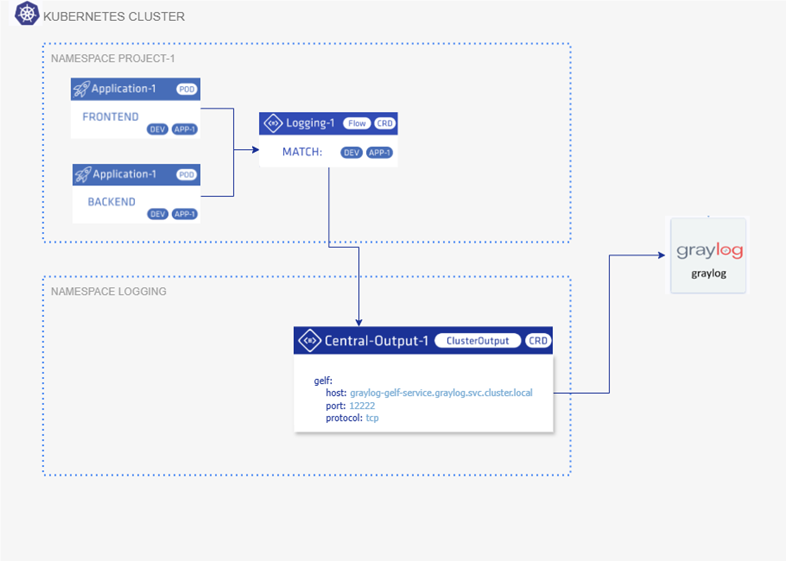
\includegraphics[scale=0.9]{img/3-background/centralized_logging/flows_output.png}
        \caption{Log Routing within Kubernetes cluster. Source: https://kube-logging.dev/docs/img/logging-operator-v2-architecture.png (adjusted) (accessed: 01.03.2025) }
        \label{fig:flows_output}
\end{figure}

\subsection{Cluster Configuration: Multiple Flows, One ClusterOutput}

To view logs in \textbf{Graylog}, create a Flow Resource on cluster:

\begin{minted}[fontsize=\small]{yaml}
    apiVersion: logging.banzaicloud.io/v1beta1
    kind: Flow
    metadata:
      name: [namespace]-flow
      namespace: [namespace]
    spec:
      filters:
        - record_transformer:
            enable_ruby: true
            records:
              - namespace: ${record["kubernetes"]["namespace_name"]}
            remove_keys: $.kubernetes.namespace_name
      globalOutputRefs:
        - cluster-output
      match:
        - select: {}
\end{minted}

\subsection{Application-Specific Logging Configuration}

All forwarded logs are enriched with additional Kubernetes metadata (Figure \ref{fig:message}). Logs arriving in Graylog in JSON-like format are automatically parsed into structured fields and stored in the following format.

\begin{figure}[h]
        \centering
        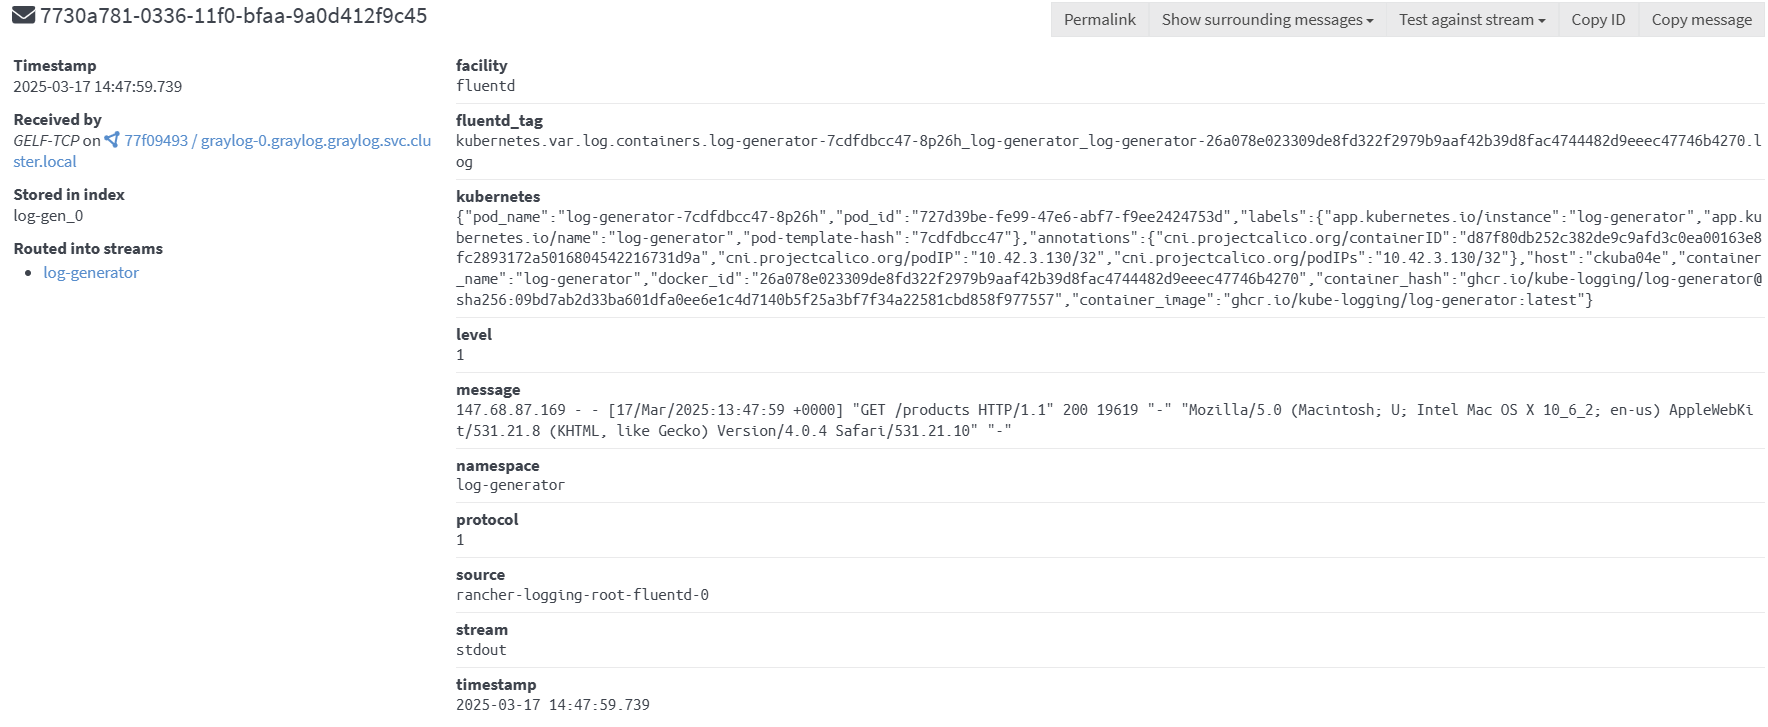
\includegraphics[scale=0.6]{img/3-background/centralized_logging/message.png}
        \caption{ }
        \label{fig:message}
\end{figure}


\begin{figure}[h]
        \centering
        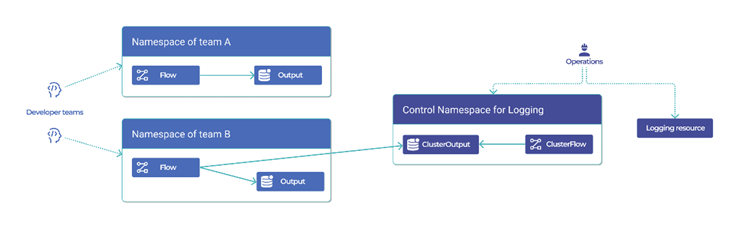
\includegraphics[]{img/3-background/centralized_logging/log_operator_flows.png}
        \caption{https://axoflow.com/wp-content/uploads/2023/11/logging-operator-multi-tenancy-2.png }
        \label{fig:log_operator_flows}
\end{figure}


\textbf{Modifying Logs}
Certain fields can be modified or removed within a Flow before storing logs in Graylog. Alternatively, logs can be forwarded unchanged and transformed directly in Graylog.

\subsection{Example Flow}
To forward all logs from a namespace, create a \textbf{Flow Resource} in the desired namespace.

\begin{itemize}
    \item If the \texttt{select} field is left empty, all logs will be forwarded.
    \item In the example below, a \textbf{filter} is applied:
    \begin{itemize}
        \item The \texttt{namespace\_name} field is extracted from the \texttt{"kubernetes"} object as a separate field.
        \item The original \texttt{namespace\_name} value in the \texttt{"kubernetes"} JSON field is removed.
    \end{itemize}
\end{itemize}

\begin{minted}[fontsize=\small]{yaml}
    apiVersion: logging.banzaicloud.io/v1beta1
    kind: Flow
    metadata:
      name: [namespace]-flow
      namespace: [namespace]
    spec:
      filters:
        - record_transformer:
            enable_ruby: true
            records:
              - namespace: ${record["kubernetes"]["namespace_name"]}
            remove_keys: $.kubernetes.namespace_name
      globalOutputRefs:
        - cluster-output
      match:
        - select: {}
\end{minted}

\textbf{Graylog Input and ClusterOutput}

The \textbf{GELF-TCP} input was created by the infrastructure team during the initial setup. The \textbf{ClusterOutput} resource forwards logs to the Graylog.

\textbf{User Administration}

Active Directory integration with Graylog was implemented to ensure that every employee can access the software. The technical application manager for Graylog grants project owners the rights to access namespaced streams. The \textbf{Project Owner} can then assign access rights to their respective team members.

\section{Perceived Value Assessment with Kano Model}

Based on the use cases described in the background chapter, the requirements expressed by the teams to assess the perceived value that Graylog brings were summarized.

\subsubsection{General Requirements for Log Management based on use cases}

\begin{enumerate}
    \item Centralized Log Aggregation

    - Collecting logs from multiple instances or microservices in chronological order to track full workflows.  

   \item Targeted Search \& Filtering
   
   - Filtering based on specific criteria (e.g., `level=error`).

   - Extract relevant fields for each specific application, such as user ID, and process them to enable log searches based on these fields.

   \item Alerting

   - Set up alerts for critical issues while avoiding unnecessary alerts (e.g., irrelevant Git merge conflicts).

   \item Quick Search

    - Provide quick search capabilities for large log volumes (e.g., GitLab).

   \item Authentication and Access Control

   - Use OpenID Connect (OIDC) with Keycloak for authentication to simplify user access management.
    
   - Centralized access control to restrict access to sensitive log data.
   
   - \gls{ad} integration for automated user management.

   \item Comprehensive Monitoring
   
   - Expand beyond log collection to include system metrics.  
   
   \item Dashboard
   
    -  Dashboards that visualize process flows, tracking logs by process ID to monitor success/failure.

    \item Efficient Storage Management
    
   - Optimize storage by sending logs to Graylog and automatically deleting them from servers.

   \item Process \& Workflow Tracing
   
   - Correlate logs across microservices to trace entire workflows.

   \item Downloading
   
   - Enable downloading of filtered logs for sharing and troubleshooting.

\end{enumerate}

To assess Graylog's perceived value, the Kano Model was used to gain insights into how different features contribute to user satisfaction. Graylog features that align with team requirements were formulated, and an evaluation was conducted to determine how these features fit into the various Kano categories based on the expressed needs of the teams.

A list of features that align with the expressed needs of the teams was compiled. The biggest focus was set on search and filtering capabilities, as failure investigation has been identified as the primary use case in the company.

Below there is a limited set of features most relevant to the use cases. While Graylog provides numerous configuration options and features, this selection was designed with consideration for users who are not yet familiar with Graylog. The features progress from basic to more sophisticated to ensure clarity and understanding, as many of them are interdependent. All listed features are taken from the open-source version Graylog Open.

\subsubsection{Selected Graylog Features}

\begin{enumerate}
    \item Automatic Input Key-Value Extraction
    \item Sidebar with list of fields
    \item Add additional field with static value
    \item Search for Field Values
    \item GROK Patterns
    \item Save Search Queries
    \item Export Search Queries to Dashboard as Widgets
    \item Custom Aggregations
    \item Real-Time Updates of Dashboards
    \item Search Time Range (Relative, Absolute)
    \item Search Time Range with Keywords
    \item Show Surrounding Messages
    \item Highlighting
    \item Alerts (Events, Notifications)
    \item Streams
    \item Pipelines
    \item Lookup Tables
    \item Decorators
    \item Export as CSV
    \item Customizable Index Sets
    \item Sidecars
    \item Content Packs (Pre-Built Setups)
    \item Authentication Service
    \item Roles
\end{enumerate}

The Kano model questionnaire will be completed using a semi-automatic tool. Each question, based on the titles from the list, will be supplemented with a description, which may include a screenshot from the Graylog application or a software architecture diagram. Additionally, a basic example will be provided, and if necessary, further use case example will be presented to illustrate how the feature can be applied in a relevant way.

\subsection{Kano questionnaire}

\end{document}